\documentclass[a4paper,12pt]{report}
\usepackage[a4paper, top=3cm, bottom=3cm, left=2.5cm, right=2.5cm]{geometry}
\usepackage[utf8]{inputenc}
\usepackage{titlesec}
\usepackage{lipsum}
\usepackage{times}
\usepackage{listings}
\usepackage{xcolor}
\usepackage{pdfpages}
\usepackage[absolute]{textpos}
\usepackage{setspace}
\usepackage{titletoc}
\usepackage[backend=biber,language=czech, sorting=none]{biblatex}
\usepackage{hyperref}
\usepackage{chngcntr}
\usepackage{csquotes}
\usepackage{tabularx}
\usepackage{pdflscape}
\hypersetup{
    colorlinks,
    citecolor=black,
    filecolor=black,
    linkcolor=black,
    urlcolor=black
}
\usepackage{dirtree}
\usepackage{jslistings}
\usepackage{prismalistings}
\usepackage{adjustbox}
\usepackage{graphicx}
\definecolor{mGreen}{rgb}{0,0.6,0}
\definecolor{mGray}{rgb}{0.5,0.5,0.5}
\definecolor{mPurple}{rgb}{0.58,0,0.82}
\definecolor{backgroundColour}{rgb}{0.95,0.95,0.92}
\definecolor{dkpurple}{rgb}{0.5, 0, 0.5}
\definecolor{dkblue}{rgb}{0,0,.6}
\definecolor{dkyellow}{cmyk}{0,0,.8,.3}

\lstdefinestyle{CStyle}{
    backgroundcolor=\color{backgroundColour},   
    commentstyle=\color{mGreen},
    keywordstyle=\color{magenta},
    numberstyle=\tiny\color{mGray},
    stringstyle=\color{mPurple},
    basicstyle=\footnotesize,
    breakatwhitespace=false,         
    breaklines=true,                 
    captionpos=b,                    
    keepspaces=true,                 
    numbers=left,                    
    numbersep=5pt,                  
    showspaces=false,                
    showstringspaces=false,
    showtabs=false,                  
    tabsize=2,
    language=C
}

\lstdefinestyle{PHPStyle}{
    language= php,
    basicstyle= \small\ttfamily,
    keywordstyle= \color{dkblue},
    stringstyle= \color{mGreen},
    identifierstyle=\color{dkpurple},
    commentstyle= \color{gray},
    emph=[1]{php},
    emphstyle=[1]\color{black},
    emph=[2]{if,and,or,else,public,function,new,return},
    emphstyle=[2]\color{dkyellow}
}

\lstdefinestyle{PythonStyle}{
    backgroundcolor=\color{backgroundColour},   
    commentstyle=\color{mGreen},
    keywordstyle=\color{magenta},
    numberstyle=\tiny\color{mGray},
    stringstyle=\color{mPurple},
    basicstyle=\footnotesize,
    breakatwhitespace=false,         
    breaklines=true,                 
    captionpos=b,                    
    keepspaces=true,                 
    numbersep=5pt,                  
    showspaces=false,                
    showstringspaces=false,
    showtabs=false,                  
    tabsize=2,
    language=Python
}
\renewcommand{\lstlistingname}{Ukázka kódu}
\renewcommand{\lstlistlistingname}{}
\renewcommand{\figurename}{Obrázek}
\renewcommand{\listfigurename}{}

% Chapter title format
\titleformat{\chapter}
  {\normalfont\fontsize{18}{21}\bfseries}{\thechapter.}{1em}{}
\titlespacing{\chapter}{0cm}{0cm}{1cm}

% Section title format
\titleformat{\section}
  {\normalfont\fontsize{15}{18}\bfseries}{\thesection}{1em}{}
\def\sectionautorefname{Kapitola}
\def\figureautorefname{Obrázek}
% For sections before table of contents
\newcommand{\unnumberedsection}[1]{%
  \section*{#1}%
}

% For section numbering
\setcounter{secnumdepth}{3}
\setcounter{tocdepth}{\value{secnumdepth}}

% Code formatting
\definecolor{codegreen}{rgb}{0,0.6,0}
\definecolor{codegray}{rgb}{0.5,0.5,0.5}
\definecolor{codepurple}{rgb}{0.58,0,0.82}
\definecolor{backcolour}{rgb}{0.95,0.95,0.92}
\lstdefinestyle{code_style}{
    backgroundcolor=\color{backcolour},   
    commentstyle=\color{codegreen},
    keywordstyle=\color{magenta},
    numberstyle=\tiny\color{codegray},
    stringstyle=\color{codepurple},
    basicstyle=\ttfamily\footnotesize,
    breakatwhitespace=false,         
    breaklines=true,                 
    captionpos=b,                    
    keepspaces=true,                 
    numbers=left,                    
    numbersep=5pt,                  
    showspaces=false,                
    showstringspaces=false,
    showtabs=false,                  
    tabsize=2,
    literate =        % Support additional characters
      {á}{{\'a}}1  {é}{{\'e}}1  {í}{{\'i}}1 {ó}{{\'o}}1  {ú}{{\'u}}1
      {Á}{{\'A}}1  {É}{{\'E}}1  {Í}{{\'I}}1 {Ó}{{\'O}}1  {Ú}{{\'U}}1
      {à}{{\`a}}1  {è}{{\`e}}1  {ì}{{\`i}}1 {ò}{{\`o}}1  {ù}{{\`u}}1
      {À}{{\`A}}1  {È}{{\`E}}1  {Ì}{{\`I}}1 {Ò}{{\`O}}1  {Ù}{{\`U}}1
      {ä}{{\"a}}1  {ë}{{\"e}}1  {ï}{{\"i}}1 {ö}{{\"o}}1  {ü}{{\"u}}1
      {Ä}{{\"A}}1  {Ë}{{\"E}}1  {Ï}{{\"I}}1 {Ö}{{\"O}}1  {Ü}{{\"U}}1
      {â}{{\^a}}1  {ê}{{\^e}}1  {î}{{\^i}}1 {ô}{{\^o}}1  {û}{{\^u}}1
      {Â}{{\^A}}1  {Ê}{{\^E}}1  {Î}{{\^I}}1 {Ô}{{\^O}}1  {Û}{{\^U}}1
      {œ}{{\oe}}1  {Œ}{{\OE}}1  {æ}{{\ae}}1 {Æ}{{\AE}}1  {ß}{{\ss}}1
      {ẞ}{{\SS}}1  {ç}{{\c{c}}}1 {Ç}{{\c{C}}}1 {ø}{{\o}}1  {Ø}{{\O}}1
      {å}{{\aa}}1  {Å}{{\AA}}1  {ã}{{\~a}}1  {õ}{{\~o}}1 {Ã}{{\~A}}1
      {Õ}{{\~O}}1  {ñ}{{\~n}}1  {Ñ}{{\~N}}1  {¿}{{?`}}1  {¡}{{!`}}1
      {°}{{\textdegree}}1 {º}{{\textordmasculine}}1 {ª}{{\textordfeminine}}1
      {£}{{\pounds}}1  {©}{{\copyright}}1  {®}{{\textregistered}}1
      {«}{{\guillemotleft}}1  {»}{{\guillemotright}}1  {Ð}{{\DH}}1  {ð}{{\dh}}1
      {Ý}{{\'Y}}1    {ý}{{\'y}}1    {Þ}{{\TH}}1    {þ}{{\th}}1    {Ă}{{\u{A}}}1
      {ă}{{\u{a}}}1  {Ą}{{\k{A}}}1  {ą}{{\k{a}}}1  {Ć}{{\'C}}1    {ć}{{\'c}}1
      {Č}{{\v{C}}}1  {č}{{\v{c}}}1  {Ď}{{\v{D}}}1  {ď}{{\v{d}}}1  {Đ}{{\DJ}}1
      {đ}{{\dj}}1    {Ė}{{\.{E}}}1  {ė}{{\.{e}}}1  {Ę}{{\k{E}}}1  {ę}{{\k{e}}}1
      {Ě}{{\v{E}}}1  {ě}{{\v{e}}}1  {Ğ}{{\u{G}}}1  {ğ}{{\u{g}}}1  {Ĩ}{{\~I}}1
      {ĩ}{{\~\i}}1   {Į}{{\k{I}}}1  {į}{{\k{i}}}1  {İ}{{\.{I}}}1  {ı}{{\i}}1
      {Ĺ}{{\'L}}1    {ĺ}{{\'l}}1    {Ľ}{{\v{L}}}1  {ľ}{{\v{l}}}1  {Ł}{{\L{}}}1
      {ł}{{\l{}}}1   {Ń}{{\'N}}1    {ń}{{\'n}}1    {Ň}{{\v{N}}}1  {ň}{{\v{n}}}1
      {Ő}{{\H{O}}}1  {ő}{{\H{o}}}1  {Ŕ}{{\'{R}}}1  {ŕ}{{\'{r}}}1  {Ř}{{\v{R}}}1
      {ř}{{\v{r}}}1  {Ś}{{\'S}}1    {ś}{{\'s}}1    {Ş}{{\c{S}}}1  {ş}{{\c{s}}}1
      {Š}{{\v{S}}}1  {š}{{\v{s}}}1  {Ť}{{\v{T}}}1  {ť}{{\v{t}}}1  {Ũ}{{\~U}}1
      {ũ}{{\~u}}1    {Ū}{{\={U}}}1  {ū}{{\={u}}}1  {Ů}{{\r{U}}}1  {ů}{{\r{u}}}1
      {Ű}{{\H{U}}}1  {ű}{{\H{u}}}1  {Ų}{{\k{U}}}1  {ų}{{\k{u}}}1  {Ź}{{\'Z}}1
      {ź}{{\'z}}1    {Ż}{{\.Z}}1    {ż}{{\.z}}1    {Ž}{{\v{Z}}}1  {ž}{{\^z}}1
      {Ž}{{\^Z}}1
}
\sloppy
\lstset{style=code_style}
\def\code#1{\texttt{#1}}
% Document metadata
\title{Webová aplikace pro rodinné úkoly}
\author{Adam Pečenka\\ 4.A\\ Informační technologie (18-20-M/01)\\}
\date{2023/2024}

% Citations
\addbibresource{references.bib}
\usepackage{chngcntr}

% Temporarly switch off page numbering
\pagenumbering{gobble}

% Title page
\begin{document}
\onehalfspacing 
\linespread{1.125}
\begin{textblock}{7}(4.5,1)
\begin{center}
\noindent \normalsize DELTA - Střední škola informatiky a ekonomie, s.r.o.\\Ke Kamenci 151, Pardubice
\end{center}
\end{textblock}
\maketitle

% Acknowledgements
\pagebreak
\unnumberedsection{Poděkování}
Chtěl bych poděkovat Ing. Monice Borkovcové, Ph.D. za vedení tohoto maturitního projektu a
konzultaci problémů. Dále bych chtěl poděkovat Jakubovi Hamplovi za pomoc se složením použitých technonologií, Nele Bartákové za pomoc se vzhledem aplikace a Martině Kozlové s Nelou Halfarovou za cennou zpětnou vazbu v rozličných oblastech.
\pagebreak

% Resumé
\pagebreak
\unnumberedsection{Anotace}
Cílem projektu je tvorba aplikace pro zadávání a plnění úkolů s webovým rozhraním.
Systém zahrnuje uživatele, kteří jsou rozděleni do skupin, které si sami zakládají, v rámci skupin si mohou sami zadat úkol sami sobě nebo jinému uživateli ve skupině. Dalším požadavkem je, aby úkoly bylo možné dělit do kategorií, které vytváří uživatelé ve skupině. Skupinu může upravit pouze její zakladatel, úkol a kategorii pouze její autor a zakladatel rodičovské skupiny. Součástí aplikace je i práce s kalendářem, kdy je možné zadat úkoly na různá období.
\unnumberedsection{Klíčová slova}
Next.js, Typescript, Prisma, tRPC, PostgreSQL, Webová aplikace, Úkoly
\unnumberedsection{Annotation}
The aim of the project is to create an application for task management with a web interface. The system includes users who are divided into groups that they create themselves. Within these groups, users can assign tasks to themselves or to other users in the group. Another requirement is that tasks can be categorized, which users within the group create. Only the founder of a group can modify it, and only the author and the founder of the parent group can modify a task and its category. The application also features calendar integration, allowing tasks to be scheduled for different time periods.

\unnumberedsection{Keywords}
Next.js, Typescript, Prisma, tRPC, PostgreSQL, Web Application, Tasks
% Název práce: Začněte názvem vaší bakalářské práce.
% Autor: Uveďte své jméno.
% Cíl práce: Stručně popište, co bylo cílem vaší práce, co jste zkoumali nebo řešili.
% Metodika: Popište, jakými metodami jste dosáhli vašich výsledků.
% Hlavní výsledky: Zdůrazněte hlavní výsledky nebo závěry vaší práce.
% Význam: Uveďte, proč jsou vaše výsledky důležité a jak mohou přispět k dané oblasti.
% Klíčová slova: Zahrňte klíčová slova nebo fráze, která charakterizují téma vaší práce.
\pagebreak

% Assignment
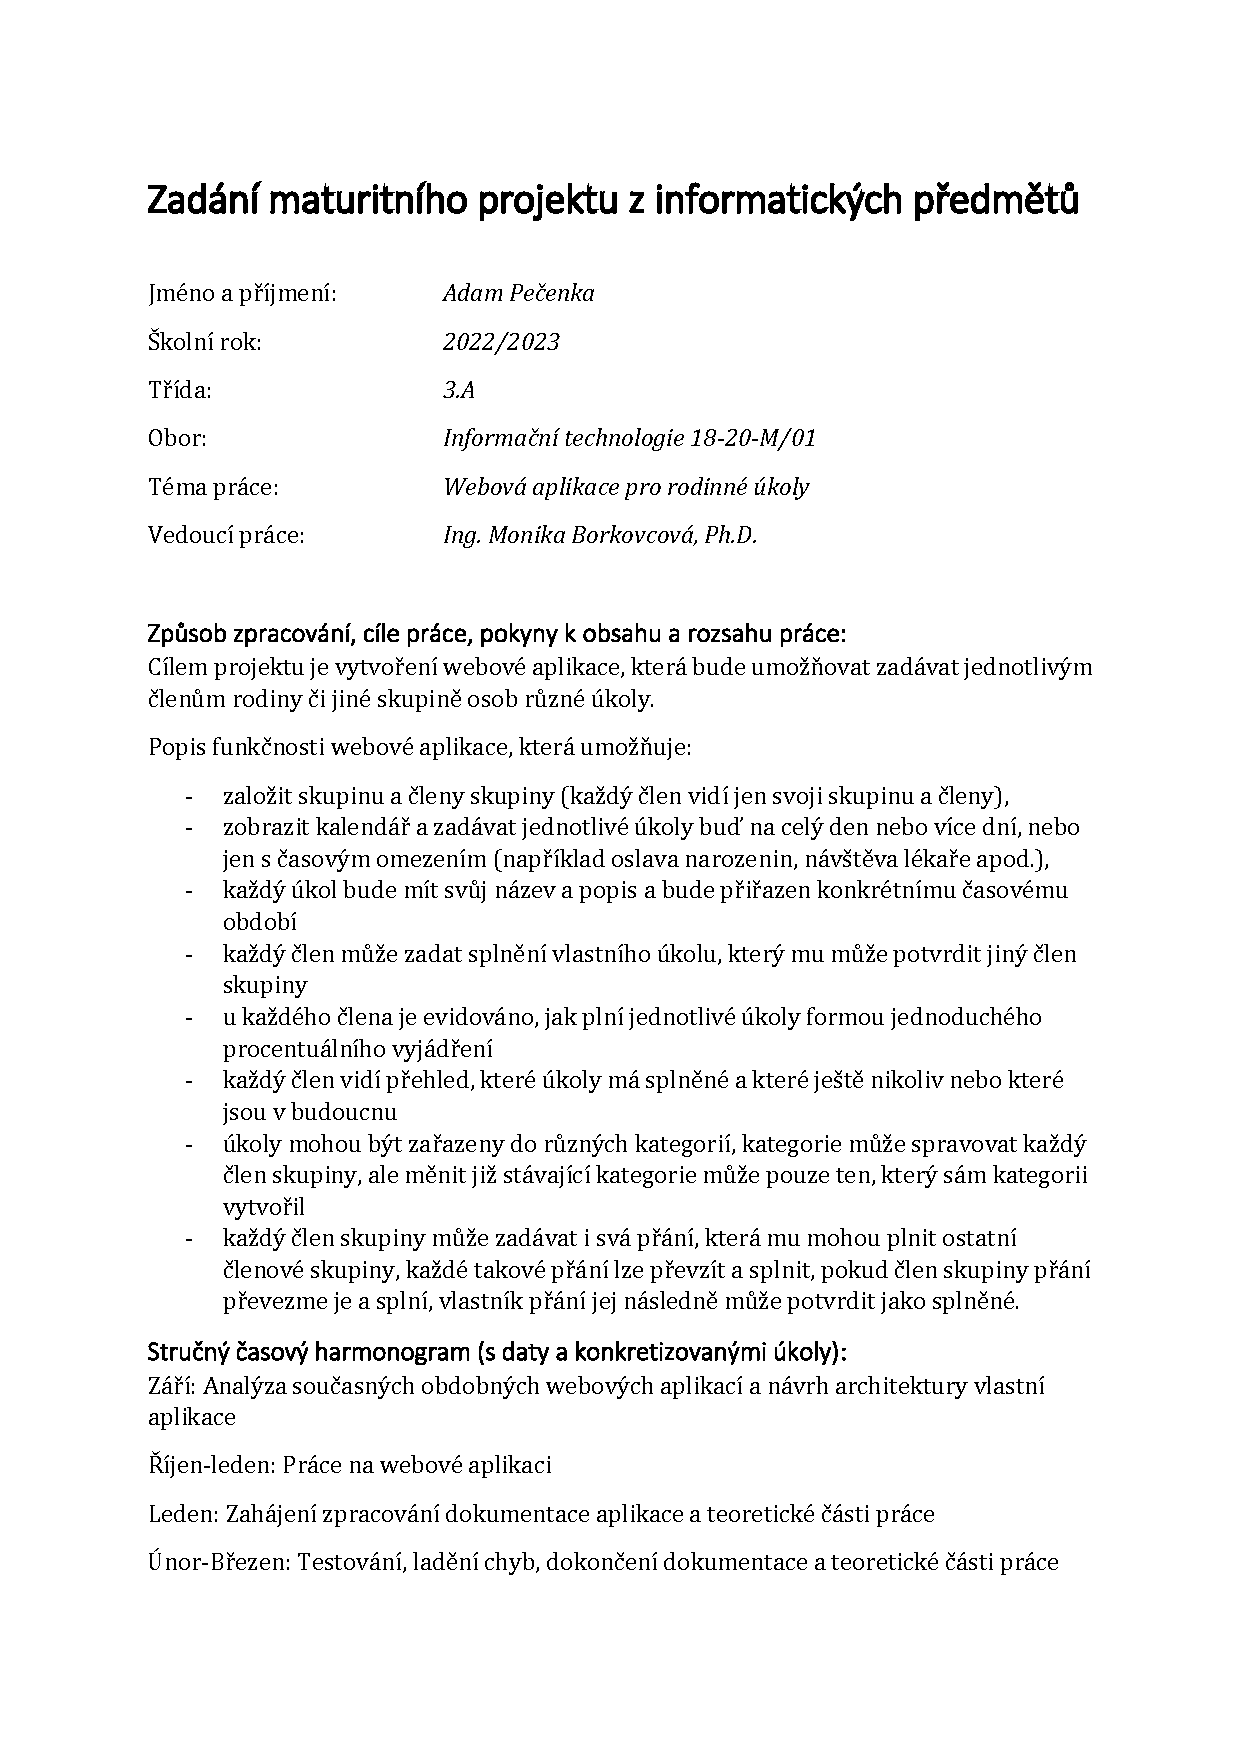
\includepdf[pages=-]{./assignment/assignment.pdf}
\pagebreak
\vspace*{\fill}
Prohlašuji, že jsem maturitní projekt vypracoval samostatně, výhradně s použitím uvedené literatury.

V Pardubicích 31.3.2024

% Acknowledgements
\pagebreak
\renewcommand{\contentsname}{\centering Obsah}
\tableofcontents
\pagebreak

% From this point onwards, switch on page numbering
\setcounter{page}{1}
\setcounter{section}{1}
\pagenumbering{arabic}
\chapter{Úvod}
V dnešní hektické době potřebuje mnoho lidí používat různé zápisníky, aby měli jistotu, že nezapomenou jak na každodenní úkoly tak na různé schůzky nebo například návštěvy u doktora. Elektronické zápisníky, tedy TODO aplikace, jsou důležité nejen pro jednotlivce, ale i pro rodiny nebo týmy ve firmách.

Cílem práce je vytvořit intuitivní TODO aplikaci s webovým rozhraním, která umožňuje rychlou správu úkolů, přání a jejich dělení do různých kategorií. Uživatelé aplikace se vzájemně přidávají do skupin ve kterých si mohou úkoly či přání zadávat.

% Content
\chapter{Porovnání s ostatními aplikacemi na trhu}
V rámci teoretické části práce jsem se před psaním vlastní "TODO" aplikace rozhodl porovnat "TODO" aplikace, které již byly uvedeny na trh. Průzkum probíhal v týdnu 15.09.2023 - 22.09.2023.
Na trhu se již vyskytuje několik velkých hráčů na trhu takzvaných "TODO"\footnote{Úkolníky} aplikací.
\section{Microsoft TODO}
Tato aplikace je jednou z populárních řešení todo aplikací pro jednotlivce. Je velmi jednoduchá na ovládání, ale nedisponuje systémem skupin, které nevyžadují rozesílání odkazů, nebo kalendářem. Uživatel si může rozdělit úkoly do jednotlivých skupin a nastavit si upozornění na jejich dokončení. Tyto upozornění jsou výhodou toho, že se jedná o .exe a ne o webovou aplikaci, a tak pro posílání upozornění nemusí mít uživatel otevřený prohlížeč. Dále aplikace disponuje určitou formou propojení s Microsoft Office 365.
\section{Trello}
Trello mířeno hlavně na týmová řešení. Je mírně komplexnější než MS TODO, ale disponuje kalendářem. Trello má dále skupiny, respektive tabule, do kterých může majitel přidávat ostatní uživatele. Uživatelé si mohou přiřadit úkoly sami nebo je může přiřadit majitel. Uživatelé si mohou zapnout sledování jednotlivých úkolů a Trello je poté informuje upozorněními na stránce.
\section{Google Keep}
Google Keep je zaměřen na osobní řešení. Uživatel má možnost provádět základní CRUDové\footnote{CRUD - Create Read Update Delete - Tvořit Číst Aktualizovat Mazat} operace na poznámkách a štítcích. Google Keep nemá funkci kalendáře či skupin, ale místo ní můžeme přidávat jako "spolupracovníky" ostatní osoby s Google účtem. I přesto, že nemá aplikace kalendář tak si uživatel může zapnout upozornění na jednotlivé poznámky.
\chapter{Technologie}
\section{Licence}
Jednou z prvních věcí kterou musíme zvážit ještě než na projektu začneme pracovat je licence pod kterou projekt bude zpracovávat. Pro projekt byla zvolena MIT Licence, také známá jako Expat nebo X11\cite{GNU-Mit}. MIT Licence vznikla na Massachusettském technologickém institutu roku 1988 a umožňuje ostatním software jakkoliv upravovat a vydávat nové verze programu, i pod jinou licencí, dokud uvedou autora a ponechají původní kód pod MIT Licencí\cite{Github-Mit}.
\section{Stack}
V dnešní době je prakticky neomezeně různých způsobů jak si sestavit technologický stack\footnote{Stack je označení pro technologie, které jsou na projektu použity} pro tvorbu full-stackové\footnote{Termín full-stack označuje aplikace, které se skládají jak z klientské části, tedy "Frontend", a ze serverové části, tedy "Backend". Backend a Frontend spolu komunikují za pomoci API.} webové aplikace.
Pro tvorbu jsem zvolil T3 Stack, T3 Stack skládá dohromady různé poměrně populární technologie na tvorbu full-stack aplikací, ale zároveň při tvoření projektu, za použití \code{create-t3-app} si umožňuje Stack jakkoliv upravit\cite{t3stack}.
\subsection{Typescript}
T3 Stack automaticky obsahuje Typescript\footnote{Zkráceně TS}, to je jedna z jeho hlavních předností, Typescript je odnož velmi populárního jazyku, pro tvorbu webových aplikací, Javascript\footnote{Zkráceně JS}. Typescript se od JS liší, jak již název napovídá, přidáním typů, byť se může zdát, že se jedná pouze o "syntaktický cukr"\footnote{Slangový termín pro nadbytečné funkce programovacích jazyků} tak je TS, narozdíl od JS, který je interpretovaný jazyk, kompilovaný jazyk.
\subsubsection{Interpretované a Kompilované jazyky}
Interpretované jazyky jsou spouštěny postupným čtením kódu od 0. řádku až na konec programu, to má za následek, že některé chyby jdou zachytit až po spuštění samotného programu. Kompilované jazyky před spuštěním projdou kompilací a mohou tak zachytit všechny chyby, které by mohly nastat.

Proces kompilace dovoluje Typescriptu zachytávat chyby, které jsou spojeny s daty co by byly typu \code{undefined} nebo \code{null}. Typ \code{undefined} se v kódu vyskytne hlavně když čekáme na data z databáze, typ \code{null} když nám databáze nic nevrátí.
Typescript je kompilovaný jazyk poměrně netradičním způsobem, protože TS se kompiluje na JS a ne na machine code\footnote{Kód, který již dokáže přečíst počítač.}.

\subsection{React a Next.js}

Celá uživatelská část aplikace je psaná pomocí nesmírně populárního frameworku Next.js, který je zároveň nadstavba snad ještě populárnějšího frameworku React. T3 Stack automaticky obsahuje Next.js, vzhledem k tomu, že prakticky nemá žádné nevýhody a poskytuje velmi příjemné funkce, které ulehčují vývoj aplikací, například automatickou optimalizaci routování nebo cachování\cite{vercel}.

\subsection{tRPC}
Pro řešení API, tedy komunikačního kanálu mezi uživatelskou a serverou částí, T3 Stack volí tRPC. tRPC je elegantní způsob jak psát endpointy\footnote{Endpoint = část API, se kterou se dá komunikovat "z venčí"}, na rozdíl od REST API nemusíme v tRPC řešit vracení statusů a postačí nám vyhodit error. Pro typovou validaci dat volí T3 stack knihovnu Zod\cite{zod}.
\begin{lstlisting}[caption={Úryvek z "groups" routeru zobrazující mazání skupiny}]
// Nerelevantní části byly nahrazeny *pseudokódem*
deleteById: protectedProcedure
    .input(z.object({ id: z.string() }))
    .mutation(async ({ ctx, input }) => {
      //*Dostaneme z databáze skupinu s identifikátorem o hodnotě id a uložíme jí do proměnné group*
      //Pokud je group o typu null nebo undefined vrátíme error
      if (!group) throw new Error("Group not found");
      //Pokud je id majitele skupiny jiné než id přihlášeného uživatele vrátíme error
      if (group.ownerId !== ctx.session.user.id)
        throw new Error("You are not the owner of this group");
      //*Smažeme skupinu v databázi*
    }),
\end{lstlisting}
Podrobnější dokumentace API se nachází níže.

\subsection{Prisma a Databáze}
Pro samotnou databázi jsem se rozhodl pro PostgreSQL, protože se jedná o velmi populární a robustní SQL Databázi.

Pro připojení na Databázi volí T3 Stack databázové ORM Prisma, v nedávných verzích přibyla možnost použití Drizzle nicméně já zvolil Prismu. Prisma je páteřní technologie, která umožňuje sdílení typů mezi serverou a klientskou částí aplikace. Další bezpochybnou výhodou Prismy je její bezpečnost, psaní čistých SQL příkazů do aplikace může vést někdy až ke kritickým chybám či ztrátě dat. Prisma ve vývojovém prostředí poskytuje našeptávání přímo z databázového schématu\footnote{Databázové schéma určuje architekturu databáze.} a tak je mnohem těžší udělat chyby.
Pro design databázového schématu používá Prisma vlastní jazyk.

\begin{lstlisting}[language=Prisma, caption={Úryvek z Databázové schématu zobrazující strukturu tabulky pro členství ve skupině}]
model GroupMembership {
  id      String @id @default(cuid())
  userId  String
  user    User   @relation(fields: [userId], references: [id], onDelete: Cascade)
  groupId String
  group   Group  @relation(fields: [groupId], references: [id], onDelete: Cascade)

  @@unique([userId, groupId])
  @@index([userId])
  @@index([groupId])
}
\end{lstlisting}
Podrobnější dokumentace celého databázového schéma se nachází níže.

\subsection{NextAuth}
Autentikaci a autorizaci užvitelů T3 Stack řeší za pomocí NextAuth. NextAuth nám umožňuje, místo standardního přihlašování email-heslo, použít takzvané \textit{Provider}y\footnote{Provider = Poskytovatel přihlášení}.
To má mnoho výhod, například, nemusíme ukládat uživatelovo heslo a přihlašování pro uživatele je jednodušší, protože mu stačí kliknout na jedno tlačítko a jeho prohlížeč ho automaticky přihlásí, za předpokladu, že už na něj přihlášený je.
Pokud přihlášený není bude poslán na přihlašovací stránku providera. NextAuth nabízí přes 30 Providerů\cite{next-auth}, já se rozhodl pro použití přihlášení od společnosti Google vzhledem k rozšířenosti Google účtů ve společnosti. Jednou z nevýhod tohoto řešení je, že pokud u vašeho Providera dojde k úniku dat budou v ohrožení i data vašich uživatelů.

\subsection{TailwindCSS, PostCSS a NextUI}
Na stylování projektu používá T3 Stack TailwindCSS. Tailwind CSS nabízí rychlou a flexibilní alternativu k psaní vanilla\footnote{Vanilla = Označení pro neupravenou verzi technologie} CSS.
\begin{lstlisting}[caption={Ukázka stylování HTML prvku za použití vanilla CSS\cite{tailwind-example}}]
//CSS soubor:
.vanilla {
  margin-top: 12px,
  margin-bottom: 12px,
  padding-left: 12px,
  padding-right: 12px
}
//HTML soubor:
<div class="vanilla"></div>
\end{lstlisting}
\begin{lstlisting}[caption={Ukázka stylování HTML prvku za použití TailwindCSS\cite{tailwind-example}}]
    <div class="mx-3 py-3"></div>
\end{lstlisting}
Než budeme moct Tailwind vůbec použít musíme vytvořit konfigurační soubor\newline\code{tailwind.config.ts}.

\begin{lstlisting}[caption={Konfigurační soubor TailwindCSS}]
import { type Config } from "tailwindcss";
import { fontFamily } from "tailwindcss/defaultTheme";
import { nextui } from "@nextui-org/react";

export default {
  content: [
    "./src/**/*.tsx",
    "./node_modules/@nextui-org/theme/dist/**/*.{js,ts,jsx,tsx}",
  ],
  theme: {
    extend: {
      fontFamily: {
        sans: ["var(--font-sans)", ...fontFamily.sans],
      },
      colors: {
        black: "#0B191E",
        cobalt: "#1D5B72",
        blue: "#043B62",
        "neon-blue": "#58C6BE",
      },
    },
  },
  darkMode: "class",
  plugins: [nextui()],
} satisfies Config;

\end{lstlisting}
Tailwind má sám o sobě velikost přibližně \code{3645 kB} to se může dát s dnešními velikostmi souborů jako málo, ale na webu je to opravdu velký soubor, proto jsem se rozhodl použít technologii PostCSS, které při stavění projektu do produkce vymaže nepoužitá stylovací pravidla z Tailwindu a sníží tím velikost jeho souboru. PostCSS se nastavuje v konfiguračním souboru \code{postcss.config.jcs}

\begin{lstlisting}[caption={Konfigurační soubor PostCSS}]
    const config = {
  plugins: {
    tailwindcss: {},
    autoprefixer: {},
  },
};

module.exports = config;
\end{lstlisting}
Tailwind nám poskytuje velkou kontrolu nad naším stylováním, ale na rozdíl od CSS frameworku Bootstrap neposkytuje předem postavené komponenty, abych tedy urychlil vývoj aplikace rozhodl jsem se použít předem stavěné komponenty za použití Tailwindu od NextUI\cite{nextui}, jmenovitě jsem použil především tabulky.

\subsection{EsLint a Prettier}
Správné formátování kódu a vyhýbání se špatným vývojovým praktikám jsou, byť snad přehlédnutelná, důležitá část jakéhokoliv projektu. Na formátování používá T3 Stack Prettier, ten v kombinaci s přídavným balíčkem do VS Code upravuje formátování při uložení souboru. Dobře naformátovaný kód ulehčuje čitelnost. Prettier se nastavuje s konfiguračním souboru \code{prettier.config.mjs}.
\begin{lstlisting}[caption=Konfigurační soubor Prettier]
/** @type {import('prettier').Config & import('prettier-plugin-tailwindcss').options} */
const config = {
  plugins: ["prettier-plugin-tailwindcss"],
};

export default config;
\end{lstlisting}
EsLint se používá na varování před praktikami, které by mohly vést k chybě a rozšiřuje tak "varovný systém", který už samotný Typescript poskytuje.
EsLint se nastavuje v konfiguračním souboru \code{.eslintrc.cjs}.


\begin{lstlisting}[caption=Konfigurační soubor EsLint]
    /** @type {import("eslint").Linter.Config} */
const config = {
  parser: "@typescript-eslint/parser",
  parserOptions: {
    project: true,
  },
  plugins: ["@typescript-eslint"],
  extends: [
    "next/core-web-vitals",
    "plugin:@typescript-eslint/recommended-type-checked",
    "plugin:@typescript-eslint/stylistic-type-checked",
  ],
  rules: {
    // These opinionated rules are enabled in stylistic-type-checked above.
    // Feel free to reconfigure them to your own preference.
    "@typescript-eslint/array-type": "off",
    "@typescript-eslint/consistent-type-definitions": "off",

    "@typescript-eslint/consistent-type-imports": [
      "warn",
      {
        prefer: "type-imports",
        fixStyle: "inline-type-imports",
      },
    ],
    "@typescript-eslint/no-unused-vars": ["warn", { argsIgnorePattern: "^_" }],
    "@typescript-eslint/no-misused-promises": [
      2,
      {
        checksVoidReturn: { attributes: false },
      },
    ],
  },
};

module.exports = config;
\end{lstlisting}
EsLint má v konfiguraci 3 možnosti hlášení, \code{off}, se hlavně používá na přepsání základních pravidel EsLintu, \code{warn}, vytvoří varování, které nikterak nebrání kompilaci kódu, \code{error}, zabrání kompilaci kódu a používá se pouze na nejzávažnější chyby\cite{eslint}.
\section{Dodatečné technlogie}
Projekt je spouštěn pomocí node.js v kombinaci s NPM. Celý kód je verzován verzovacím systémem Git a psán v textovém editoru Visual Studio Code.
\subsection{package.json}
Tento konfigurační soubor je často přehlížen, ale jedná se o stěžejní konfigurační soubor celého projektu. V \code{package.json} jsou definovaný takzvané "závislosti" projektu. \code{Package.json} ve své podstatě funguje jako nákupní seznam kde máme právě tyto závislost napsané. Když naklonujeme projekt tak jedna z prvních věcí co musíme udělat je spustit příkaz \code{npm i}, ten vezme \code{package.json} a z platformy NPM\cite{npm} stáhne všechny balíčky na kterých projekt závisí a automaticky je nainstaluje do složky \code{node\_module}.
\section{Konfigurace}
Ještě než se nám podaří spustit projekt musíme vytvořit konfigurační soubor \code{.env}\footnote{Z anglického "enviorement", tedy "prostředí"}. Ten z bezpečnostních důvodů není obsažen v repozitáři, protože obsahuje velmi citlivé informace jako přístupové údaje k databázi nebo klíče k autentikaci uživatelů. Vzhledem k tomu, že \code{.env} soubor musí mít pro správné fungování aplikace jistou strukturu je v repozitáři šablona \code{.env.example}. Následuje soubor \code{.env.example}, komentáře v souboru byly vynechány.
\begin{lstlisting}[caption=Šablona konfiguračního souboru .env]
...
# Prisma
...
DATABASE_URL=""
DATABASE_NON_POOLING_URL=""

# Next Auth
...
NEXTAUTH_SECRET=""
NEXTAUTH_URL=""

# Next Auth Providers
GOOGLE_CLIENT_ID=""
GOOGLE_CLIENT_SECRET=""
\end{lstlisting}
\chapter{Aplikace}
Vzhledem ke komplexnosti aplikace je pro přehlednost rozdělena do několik složek.
\section{Prisma}

Databázové schéma v jazyku Prisma a databázové migrace se nachází ve složce \code{/prisma/}. Po úpravě Databázové schématu je dobré i vytvořit databázovou migraci, ta nám umožní manuálně spustit SQL příkazy, které Prisma vykonala pokud to bude potřeba.
Následuje vizualizace Databázové schématu vygenerovaná pomocí webové aplikace Prismaliser \cite{prismaliser}.
\begin{figure}[hbt!]
    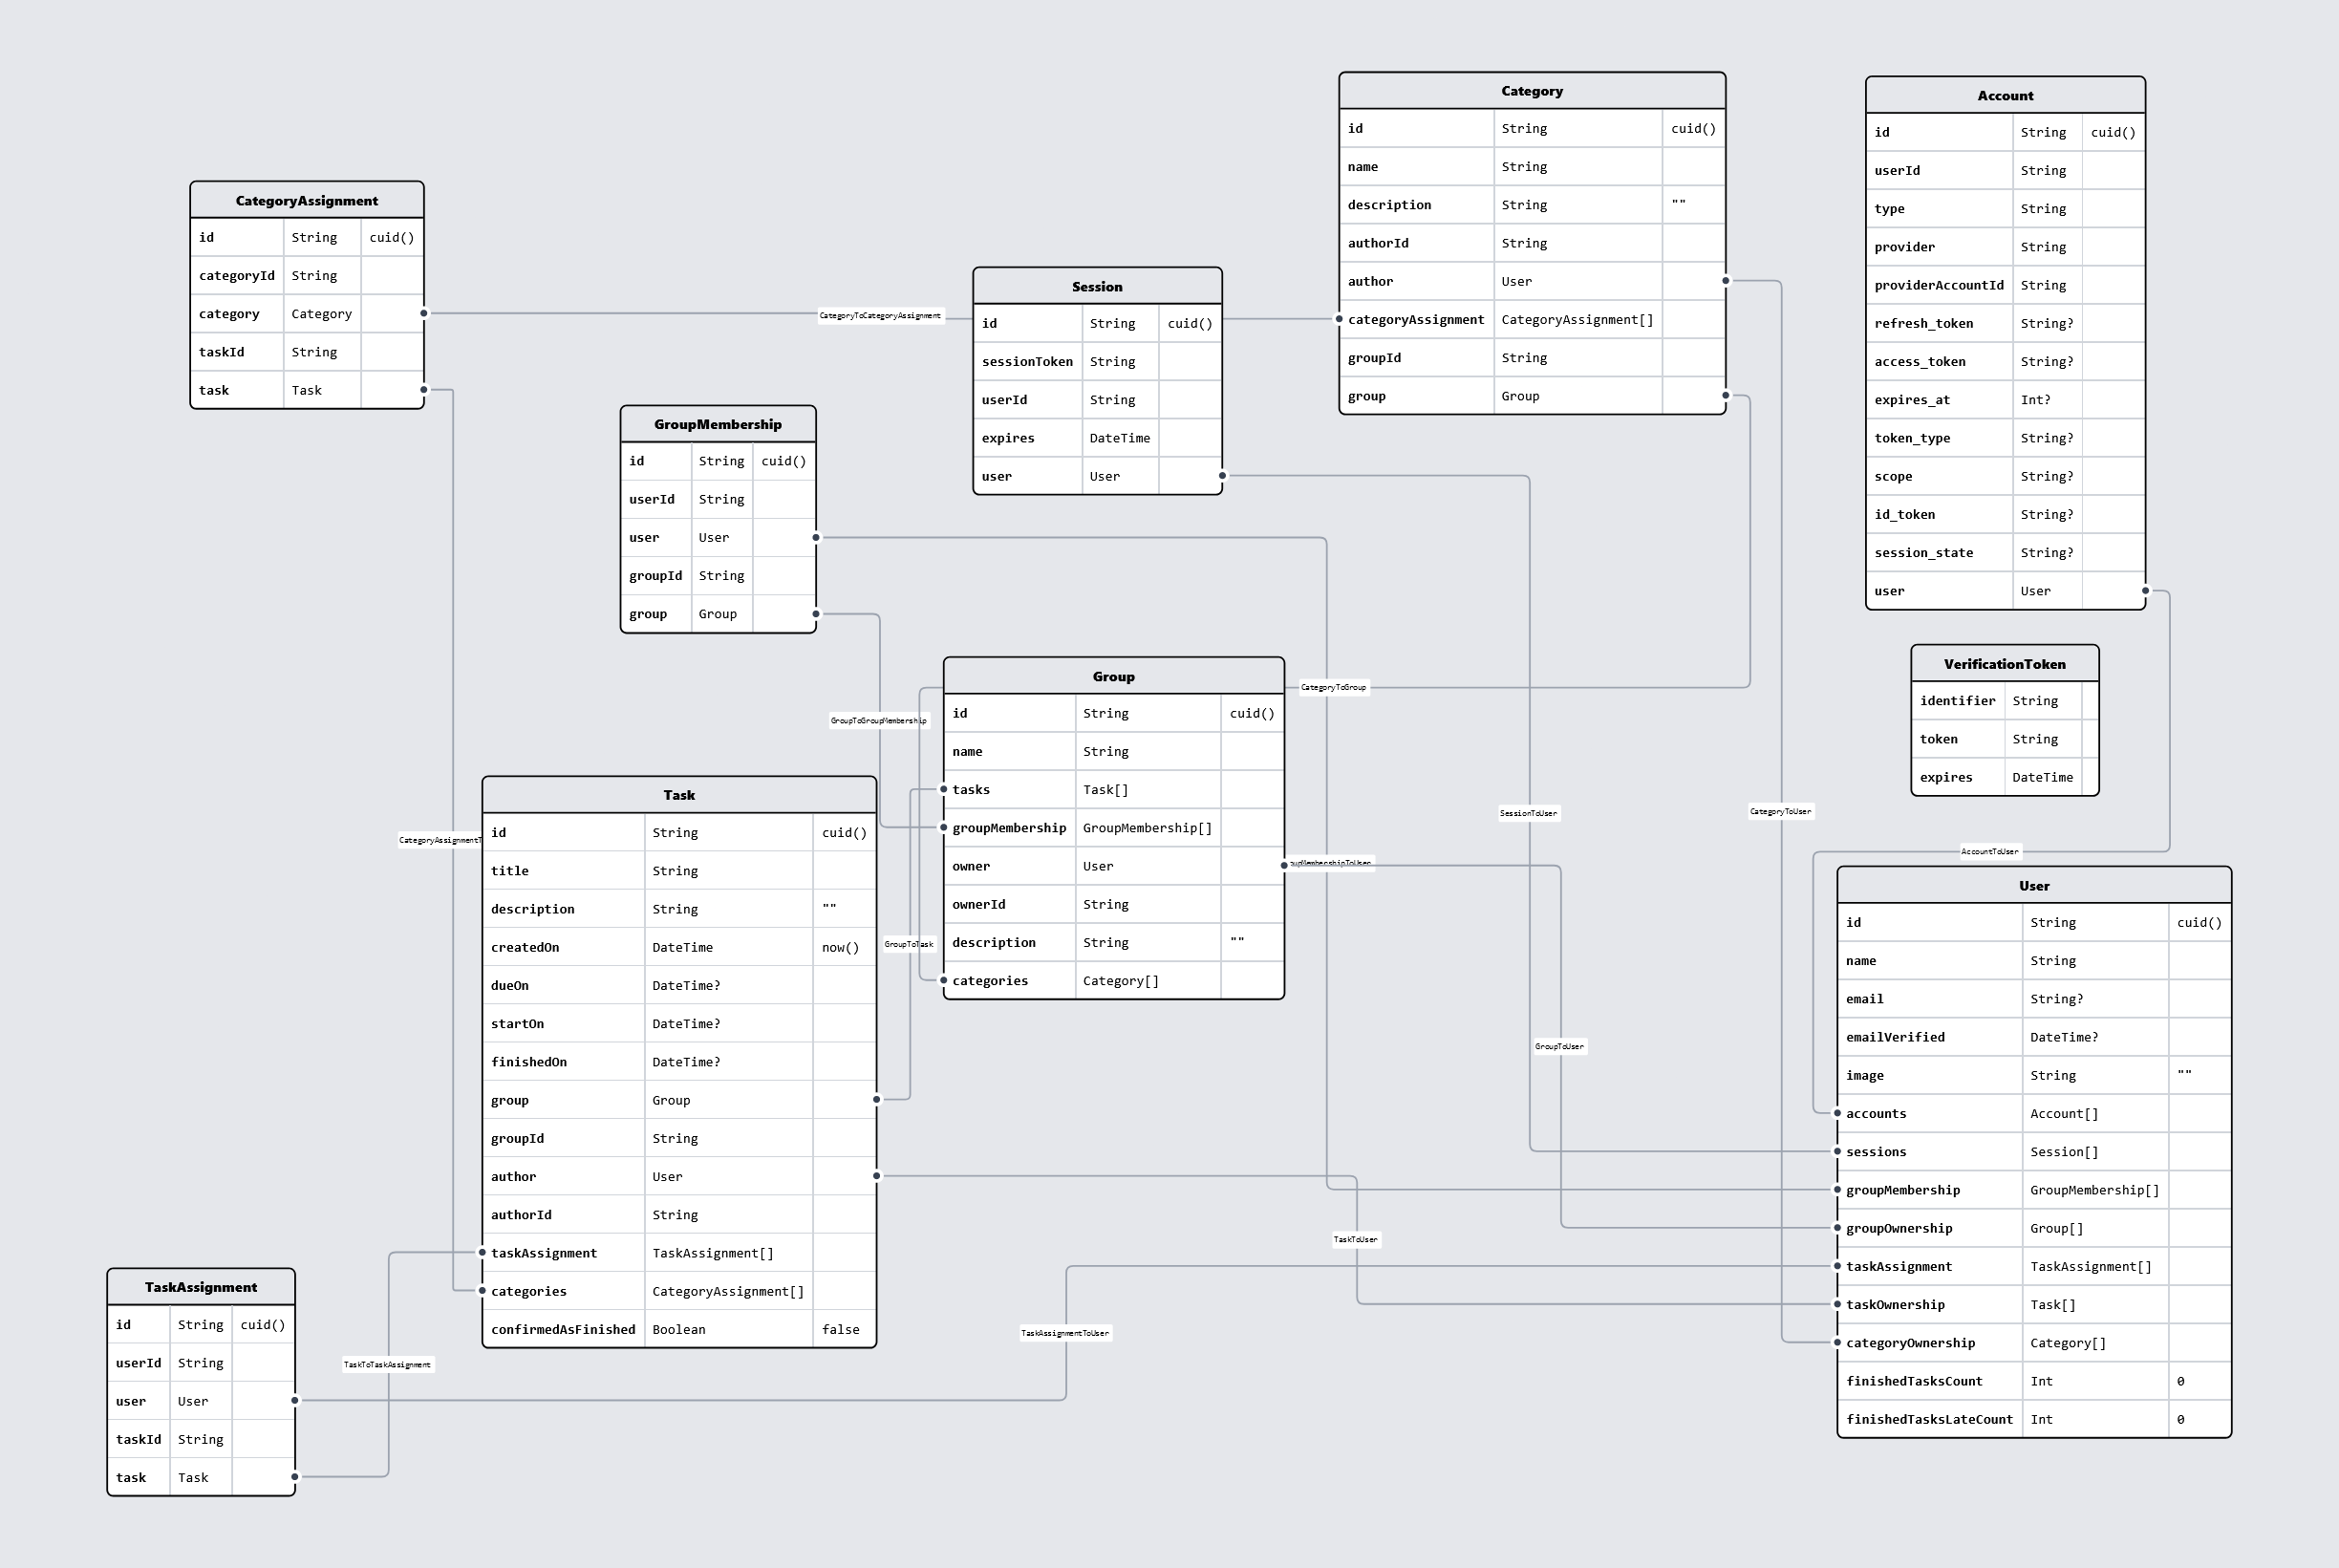
\includegraphics[width=1\linewidth]{img/DB_schema.png}
    \caption{Databázové schéma}
\end{figure}
\section{API}
Jak již zaznělo, celé API je psané za pomocí tRPC, to se nachází ve složce \code{/src/server/api/}.
API je inicializováno v souborech \code{trpc.ts} a \code{root.ts}. Konktrétně v souboru \code{trpc.ts} inicializujeme objekt tRPC a v \code{root.ts} na něj napojujeme jednotlivé Routery. Samotné "Endpointy", tedy přístupy, jsou rozděleny do "Routerů", ty se nachází ve složce \code{/src/server/api/routers} a dělí se na jednotlivé "hlavní objekty" v databázi. Tyto routery jsou děleny na soubory \code{categories.ts}, \code{groups.ts}, \code{tasks.ts} a \code{users.ts}. V kódu se "Endpointy" označují jako "Procedury", v princpu existují dva druhy procedur; Public\footnote{Veřejná} a Protected\footnote{Chráněná}. Jediným rozdílem mezi nimi je, že Protected procedura zaručuje, že jí může úspěšně zavolat pouze přihlášený uživatel.
Následuje úryvek z Routeru pro skupiny v souboru \code{groups.ts}. Ostatní procedury byly z ukázky odstraněny.
\begin{lstlisting}[caption={Procedura na přidání uživatele do skupiny}]
import { z } from "zod";

import {
  createTRPCRouter,
  protectedProcedure,
  publicProcedure,
} from "~/server/api/trpc";

export const groupsRouter = createTRPCRouter({
...
addMember: protectedProcedure
    .input(z.object({ userId: z.string(), groupId: z.string() }))
    .mutation(async ({ ctx, input }) => {
      const group = await ctx.prisma.group.findFirst({
        where: { id: input.groupId },
      });
      if (!group) throw new Error("Group not found");
      const user = await ctx.prisma.user.findFirst({
        where: { id: input.userId },
      });
      if (!user) throw new Error("User not found");
      if (group.ownerId !== ctx.session.user.id)
        throw new Error("You are not the owner of this group");
      const membership = await ctx.prisma.groupMembership.create({
        data: {
          groupId: input.groupId,
          userId: input.userId,
        },
      });
      if (membership) return true;
      return false;
    }),
...
})
\end{lstlisting}
Jako první musíme definovat název Procedury, v tomto případě "addMember", tedy "přidatUživatele". Dále přidáme \code{.input()} zde bude přijímat procedura data pro své provedení. Pokud bude Procedura data měnit tak přidáme \code{.mutation}, pokud data pouze předá z Databáze tak přidáme \code{.query}. Do těch poté předáme vstup z \code{.input} a \code{ctx}\footnote{Kontext}. Kontext je globálně zpracovávaný a nachází se v něm \code{session} přihlášeného uživatele a \code{prisma}, tou se napojujeme na databázi.
\subsection{Příklad API Endpointů}
    \begin{tabularx}{1\textwidth} { 
  | >{\centering\arraybackslash}X 
  | >{\centering\arraybackslash}X 
  | >{\centering\arraybackslash}X 
  | >{\centering\arraybackslash}X 
  | >{\centering\arraybackslash}X | }
     \hline
        \textbf{Router} & \textbf{Název} & \textbf{Popis} & \textbf{Vstup} & \textbf{Výstup}\\
         \hline
         tasks.ts & assignUser & Přiřadí uživatele k úkolu & ID uživatele, ID úkolu & True / False\\
          \hline
         tasks.ts & getCategories & Vrátí pole kategorií úkolu & ID úkolu & Category[]\\
         \hline
         groups.ts & getById & Vrátí objekt skupiny pokud je přihlášený uživatel člen & ID skupiny & Group\\
         \hline
         groups.ts & leave & Odstraní přihlášeného uživatele ze skupiny & ID skupiny & True / False\\
         \hline
         users.ts & locateByName & Vrátí pole uživatelů s podobným jménem k vstupu & Text & User[]\\
         \hline
         users.ts & editName & Upraví jméno uživatele & ID uživatele, Nové jmnéno & User\\
         \hline
         categories.ts & create & Vytvoří kategorii & Název, Popis, ID autora, ID skupiny & Category\\
         \hline
         categories.ts & getTasks & Vrátí úkoly s kategorií & ID kategorie & Task[]\\
         \hline
    \end{tabularx}

\chapter{Závěr}
V rámci maturitní práce vznikla aplikace splňující všechny body v zadání, nad rámec zadání byl přidán Streak systém. Aplikace je hostovaná na platformě Vercel\cite{vercel} a databáze je hostovaná na platformě Neon\cite{neon}. Aplikace disponuje správou skupin, úkolů a kategorií. Každý uživatel má přístup pouze do do skupin ve kterých je členem, k úkolům a kategoriím má přístup pouze pokud je členem rodičovské skupiny. Veškerá uživatelem generovaná data mohou být upravovaná tím kdo je vytvořil, kromě úkolů a kategorií, ty může upravovat jejich autor a majitel rodičovské skupiny. 
% Literature
\chapter{Přílohy}
\begin{landscape}
\section{Class diagramy}

% Vypadá na to na prd, ale lepší už to nebude.
\begin{figure}[hbt!]
	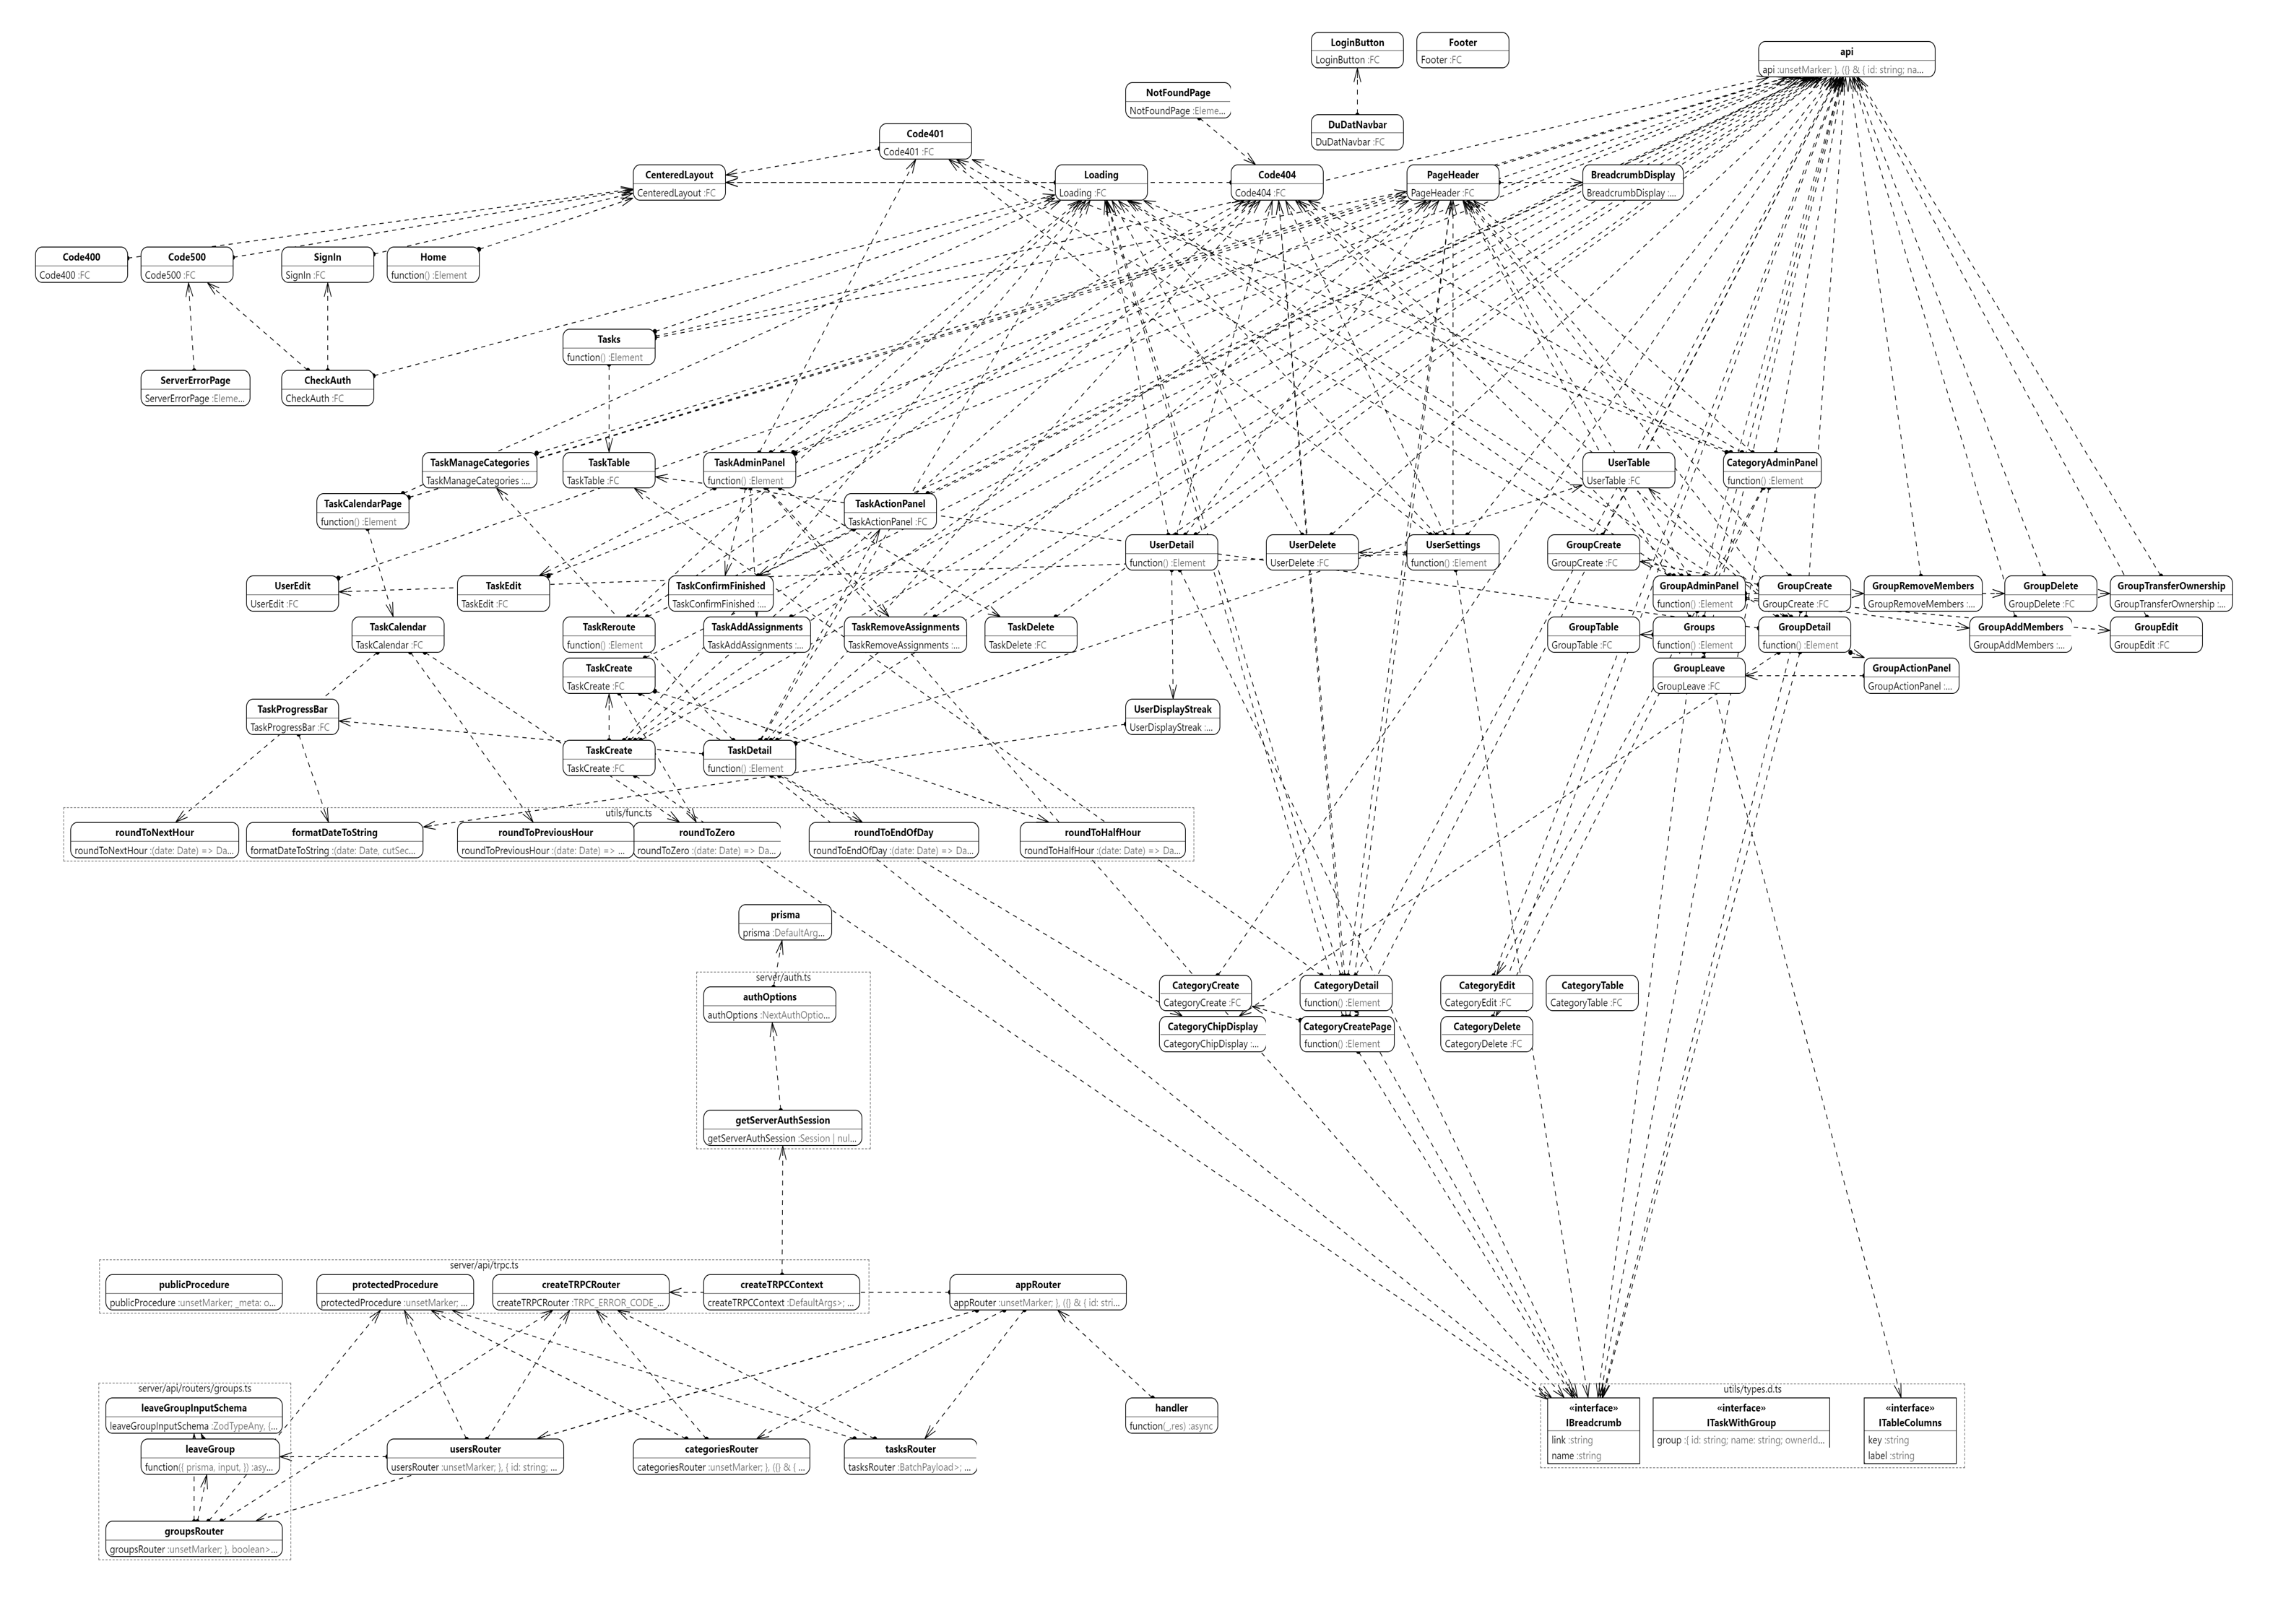
\includegraphics[width=1\linewidth, height=0.55\linewidth]{img/ClassDiagramy/src_diagram_export.png}
	\caption{Class diagram projektu}
	\label{fig:enter-label}
\end{figure}
\pagebreak
\begin{figure}[hbt!]
	\centering
	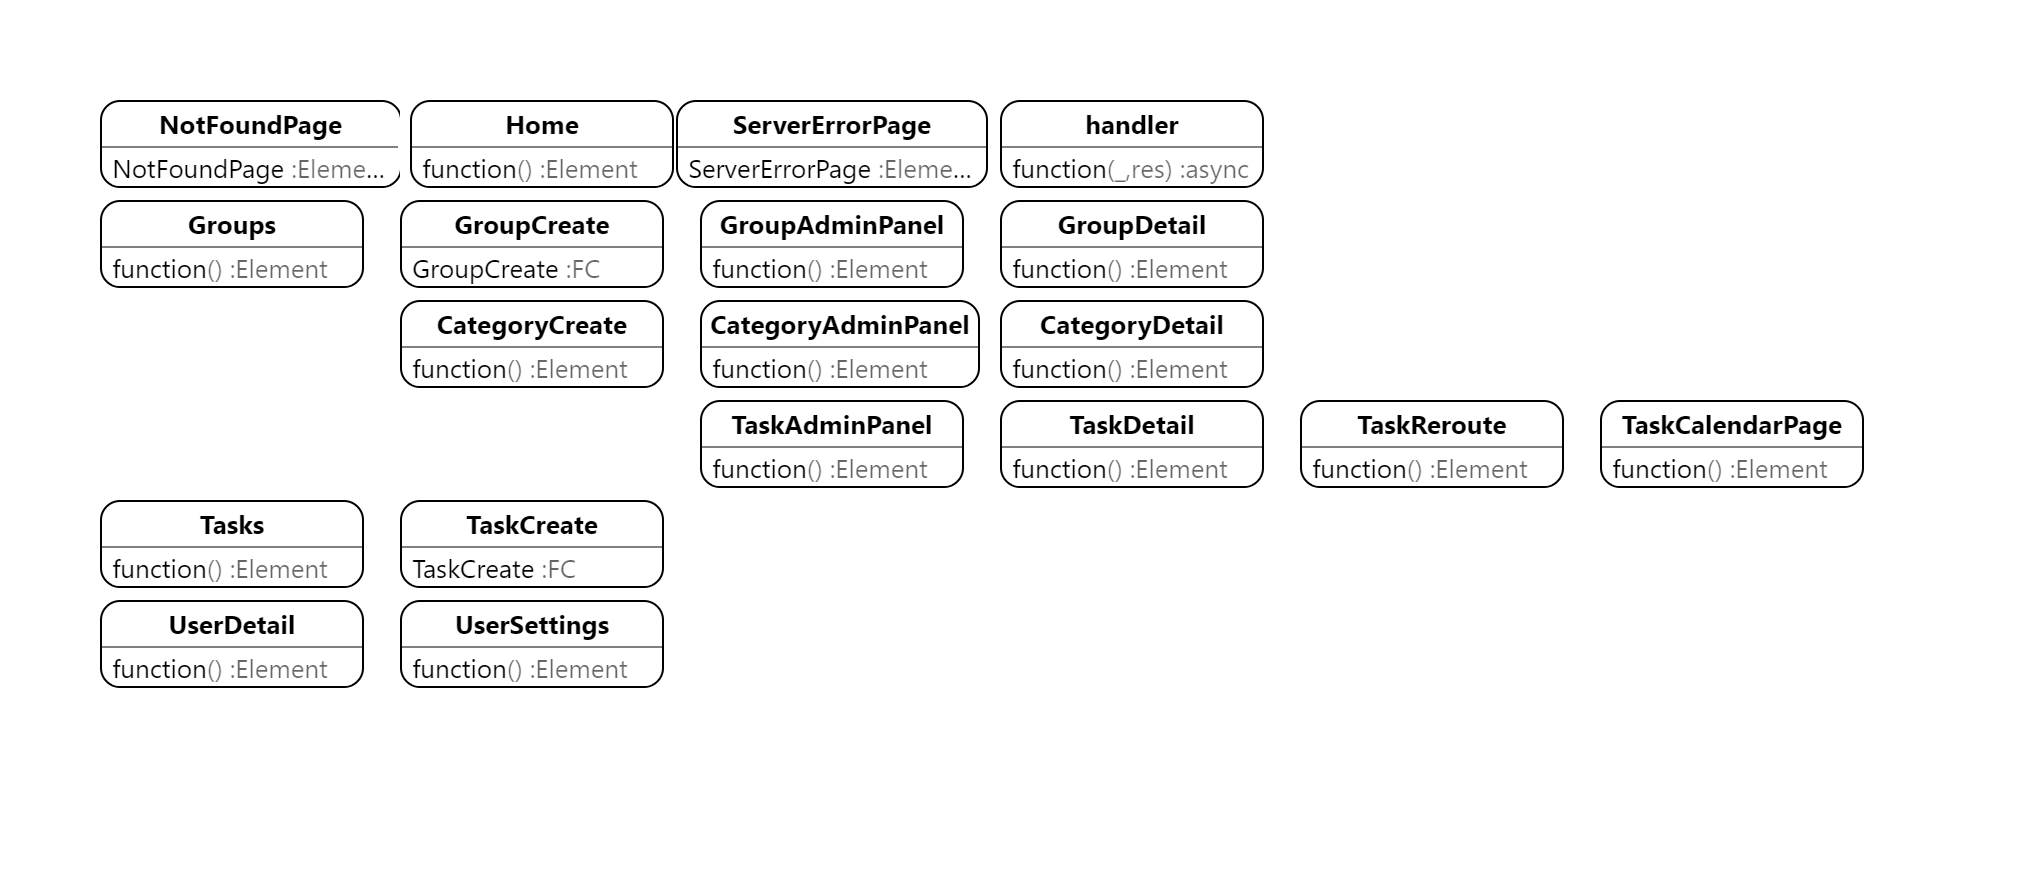
\includegraphics[width=1\linewidth]{img/ClassDiagramy/pages_diagram.png}
	\caption{Class diagram stránek}
\end{figure}
\begin{figure}[hbt!]
	\centering
	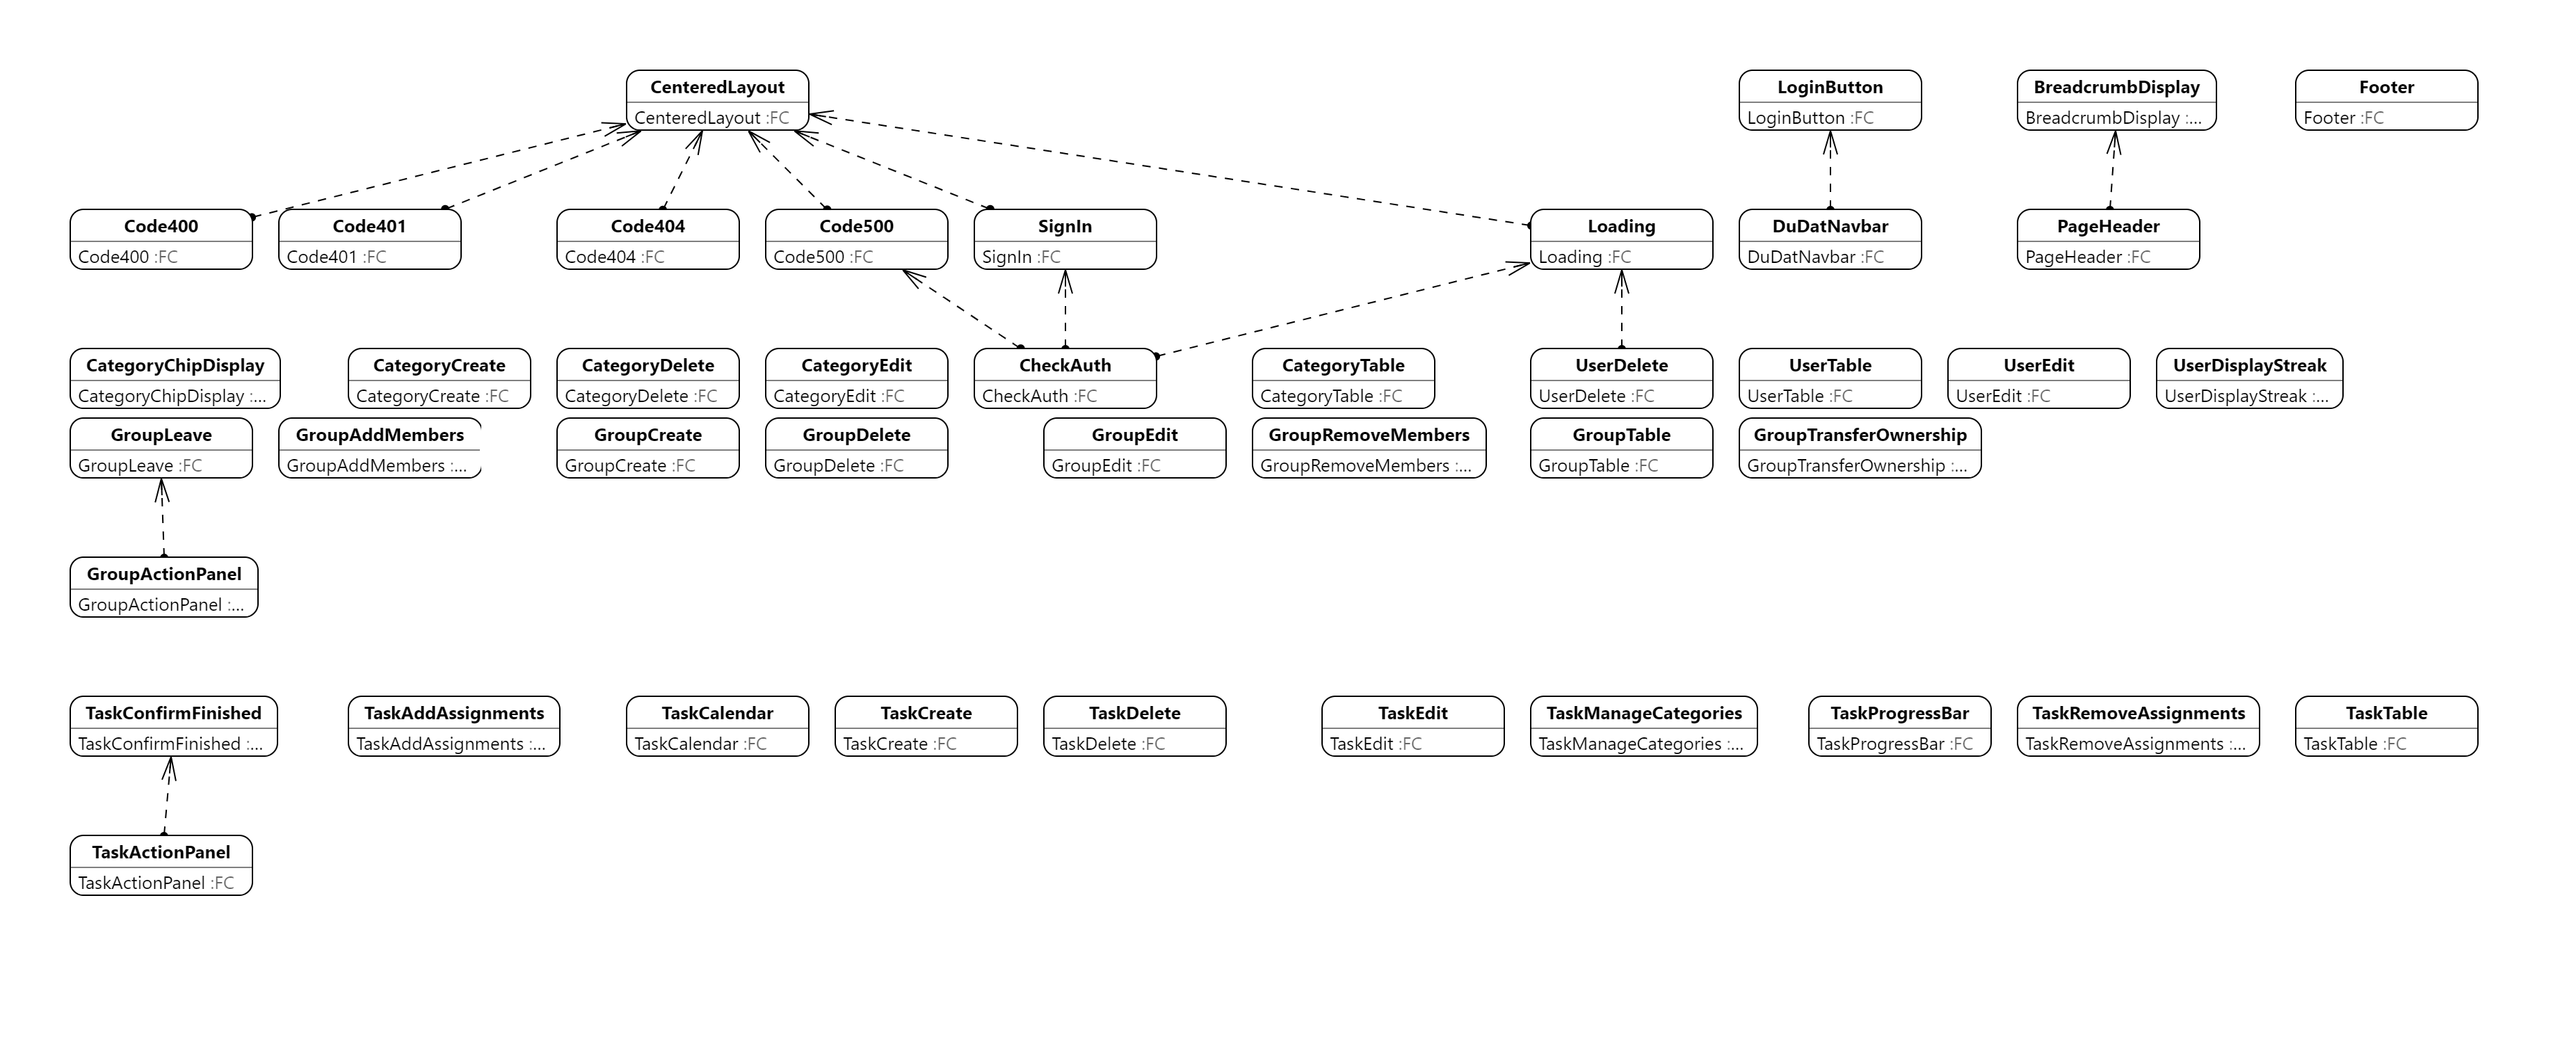
\includegraphics[width=1\linewidth]{img/ClassDiagramy/components_diagram.png}
	\caption{Class diagram komponent}
\end{figure}
\pagebreak
\begin{figure}[hbt!]
	\centering
	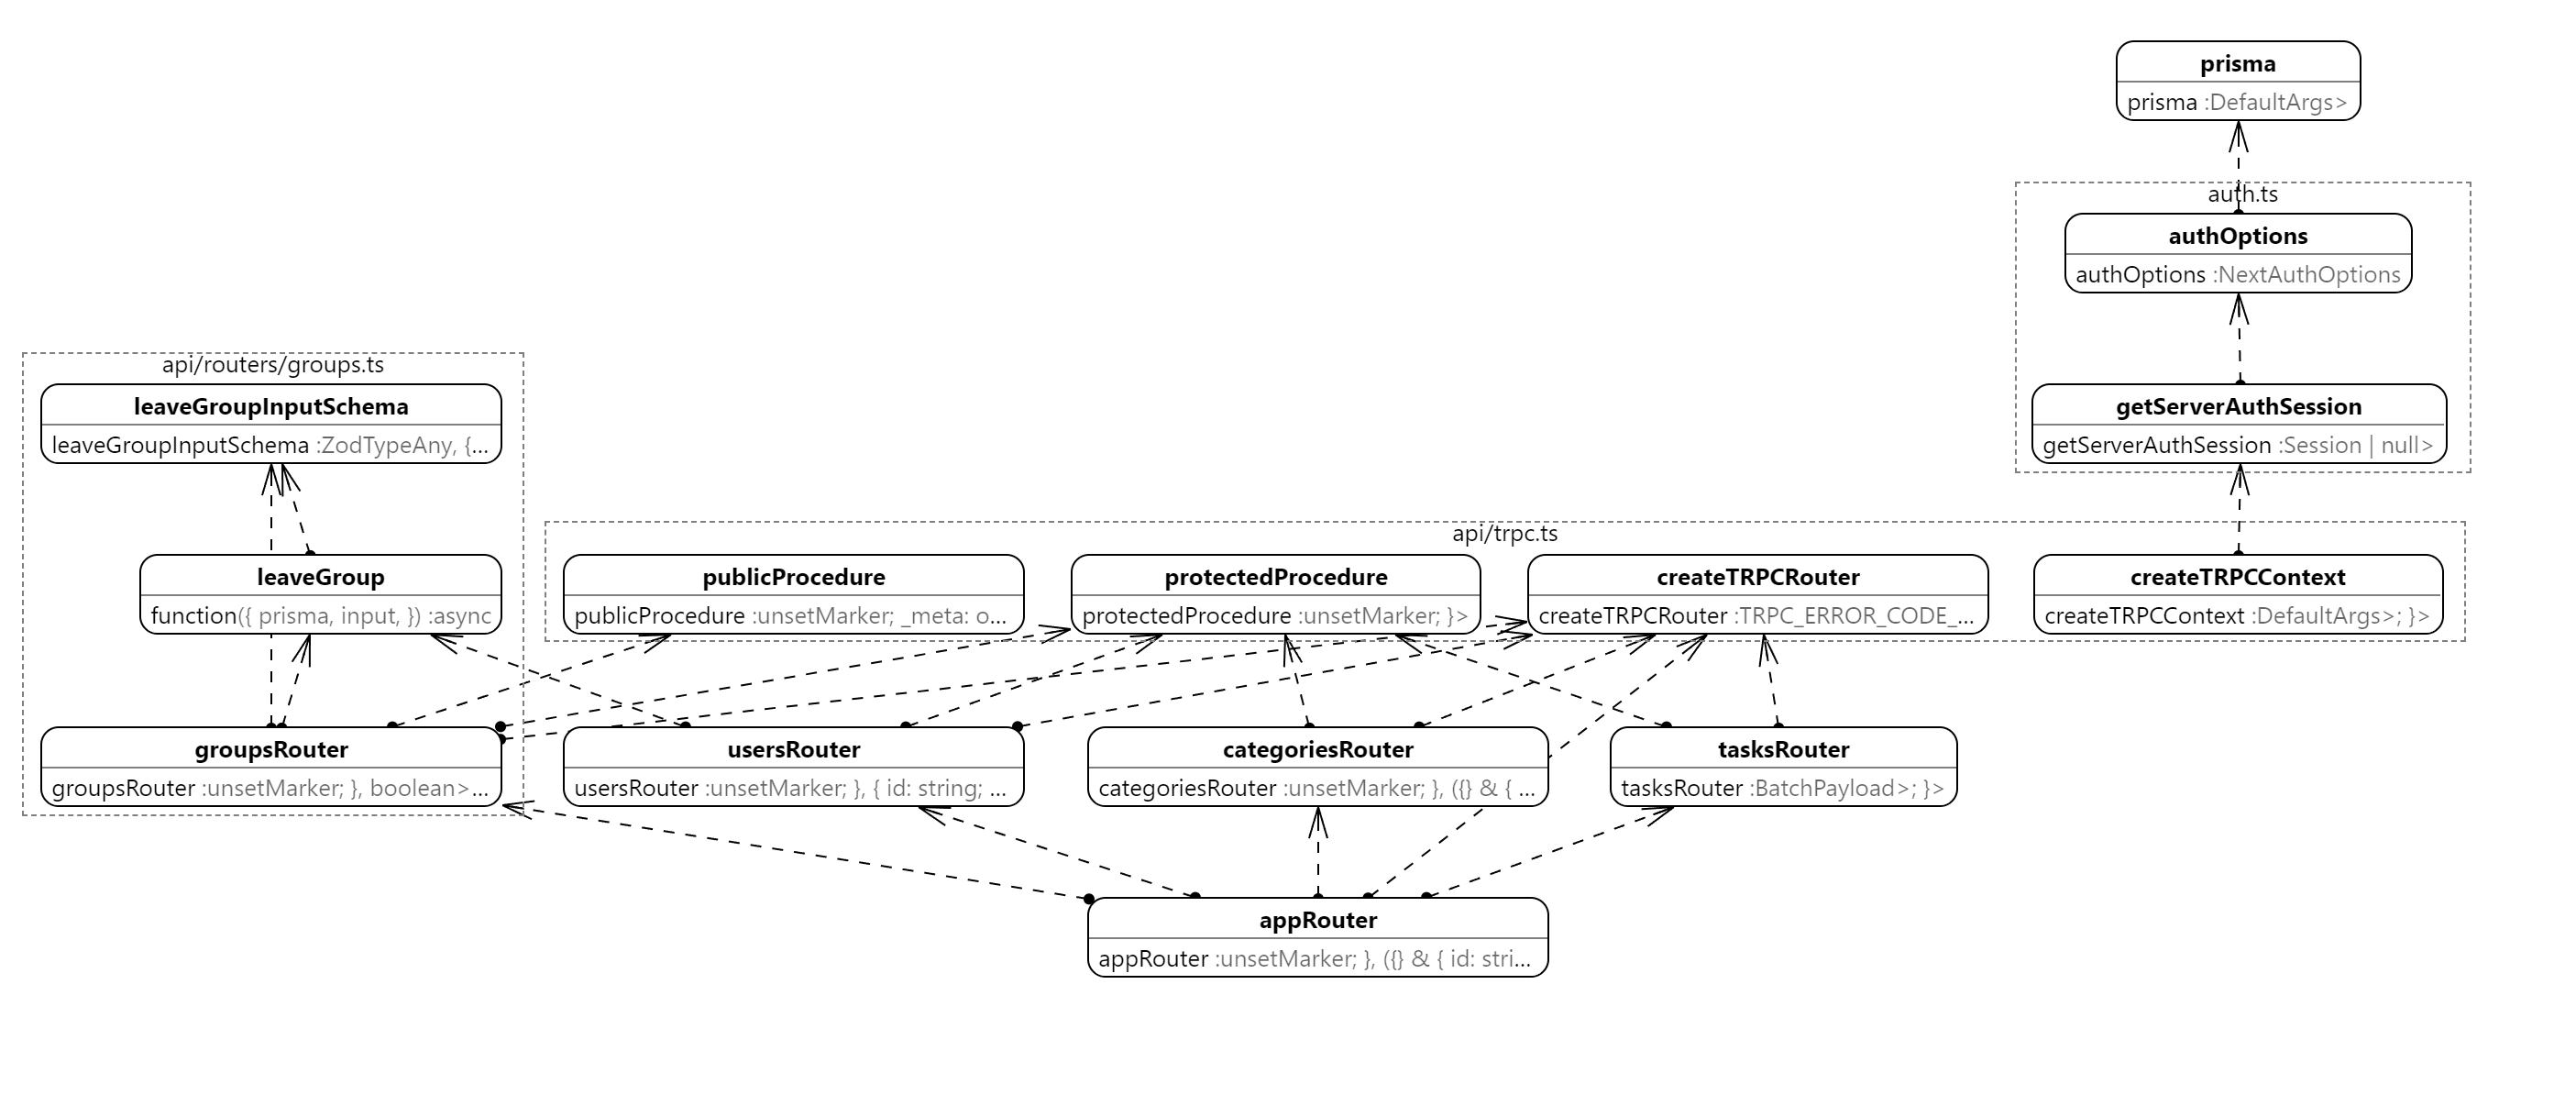
\includegraphics[width=1\linewidth]{img/ClassDiagramy/server_diagram.png}
	\caption{Class diagram serverové části aplikace}
\end{figure}
\begin{figure}[hbt!]
	\centering
	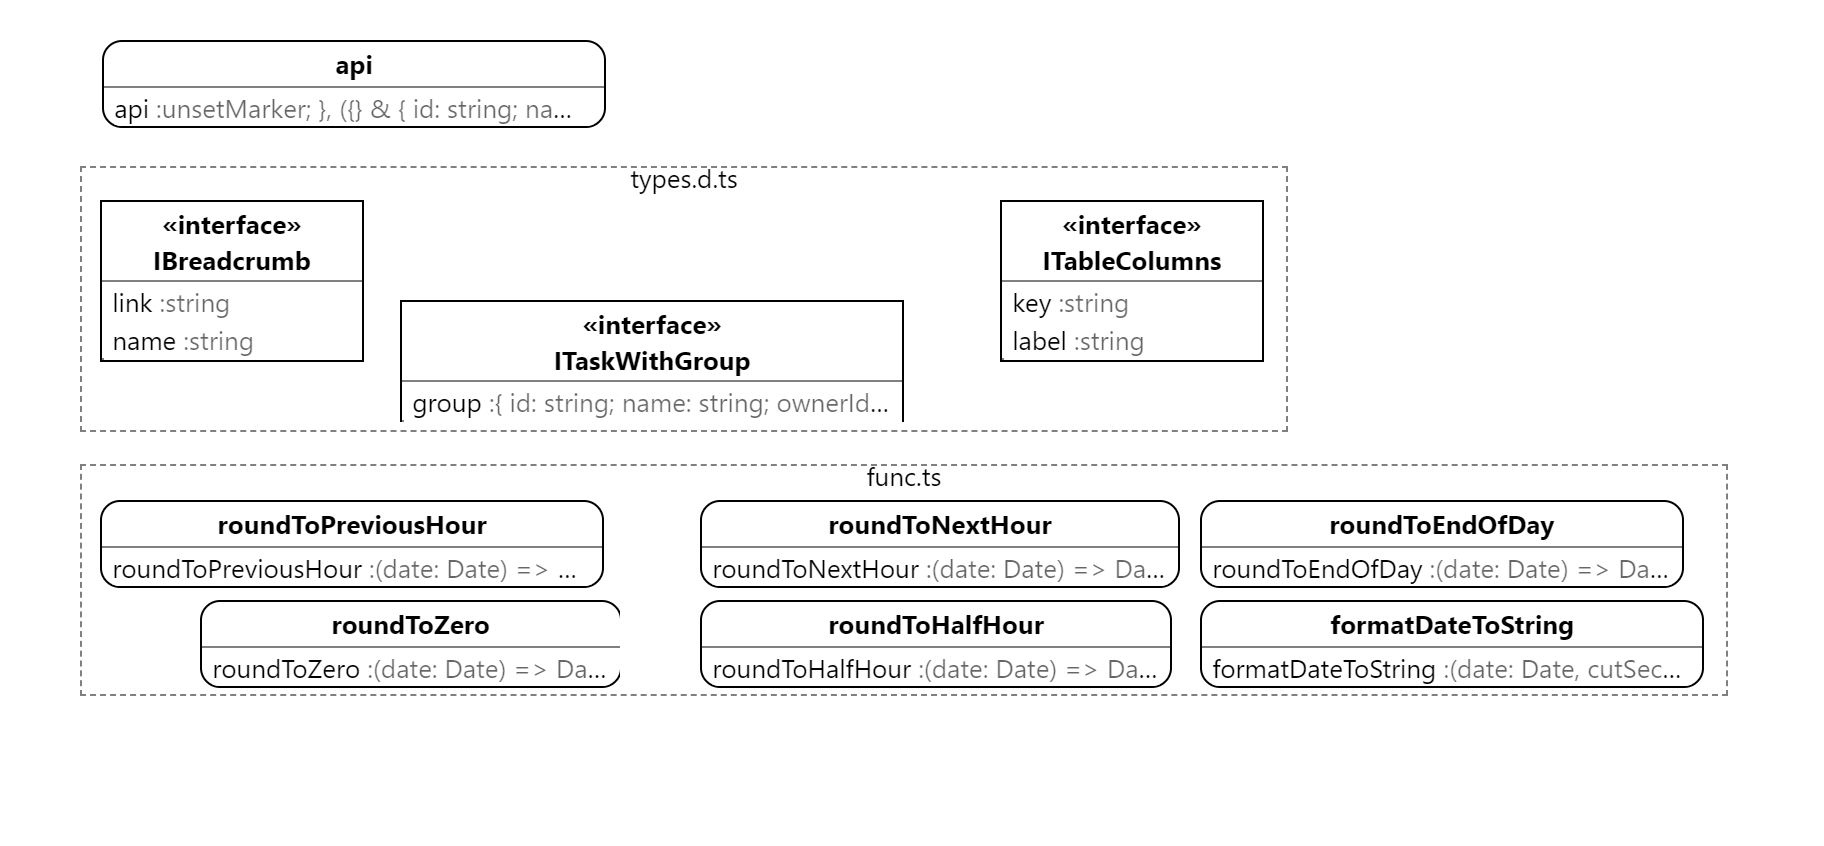
\includegraphics[width=1\linewidth]{img/ClassDiagramy/utils_diagram.png}
	\caption{Class diagram podpůrných funkcí a rozhraní}
\end{figure}

\pagebreak
\end{landscape}
\let\clearpage\relax
\section{Literatura}
\printbibliography[heading=none]
\pagebreak
\section{Obrázky}
\vspace{-64pt}
\listoffigures
\pagebreak
\section{Ukázky}
\vspace{-48pt}
\lstlistoflistings

\pagebreak

\end{document}